\documentclass{beamer}
\usepackage[english, russian]{babel}
\usepackage[T2A]{fontenc}
\usepackage[utf8]{inputenc}
\usepackage{indentfirst}
\usepackage{amsmath, amsfonts, amssymb, amsthm, mathtools}
\usepackage[export]{adjustbox}
\usepackage{graphicx} 
\graphicspath{ {./images/} }

\usepackage{subcaption}
\usepackage{verbatim}

\usepackage{minted}{\setlength{\parskip}{0pt}}

\usepackage{hyperref}

\hypersetup{
    colorlinks=true,
    linkcolor=blue,
    filecolor=magenta,      
    urlcolor=black,
    pdftitle={Overleaf Example},
    pdfpagemode=FullScreen,
    }


\title{Лабораторная работа № 5. \\ Расширенная настройка HTTP-сервера Apache}
\author{Данила Стариков \\ НПИбд-02-22}
\institute{Российский университет дружбы народов имени Патриса Лумумбы}
\date{2024}

\begin{document}

\frame{\titlepage}

\begin{frame}
\frametitle{Цель работы}
\begin{itemize}
    \item Приобретение практических навыков по расширенному конфигурированию HTTP-сервера Apache в части безопасности и возможности использования PHP.
\end{itemize}
\end{frame}

\begin{frame}[containsverbatim]
\frametitle{Конфигурирование HTTP-сервера для работы через протокол HTTPS}
Сгенерировали ключ и сертификат, используя следующую команду:
\begin{minted}{bash}
openssl req -x509 -nodes -newkey rsa:2048 -keyout www.dastarikov.net.key -out www.dastarikov.net.crt
mv www.dastarikov.net.crt /etc/pki/tls/certs
    \centering
    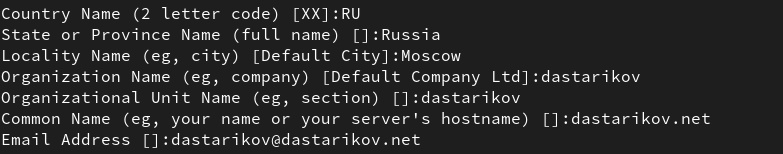
\includegraphics[width=\textwidth]{../images/image01.png}
    \captionof{figure}{Создание SSL-сертификата.}
\end{frame}

\begin{frame}
\frametitle{Конфигурирование HTTP-сервера для работы через протокол HTTPS}
    \centering
    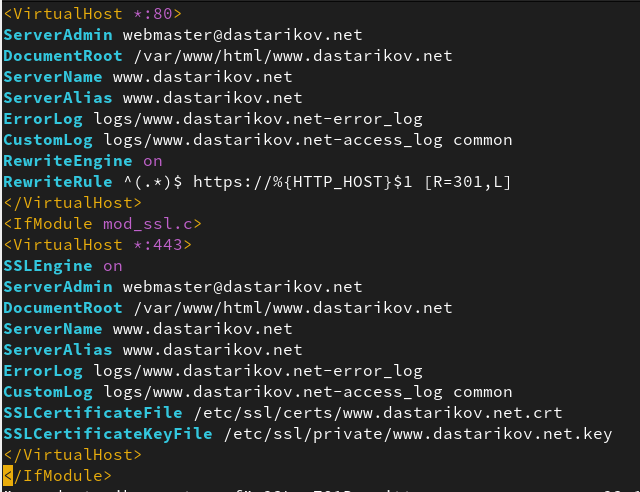
\includegraphics[width=0.8\textwidth]{../images/image03.png}
    \captionof{figure}{Изменение конфигурационного файла для работы через протокол HTTPS.}
\end{frame}

\begin{frame}
\frametitle{Конфигурирование HTTP-сервера для работы через протокол HTTPS}
    \centering
    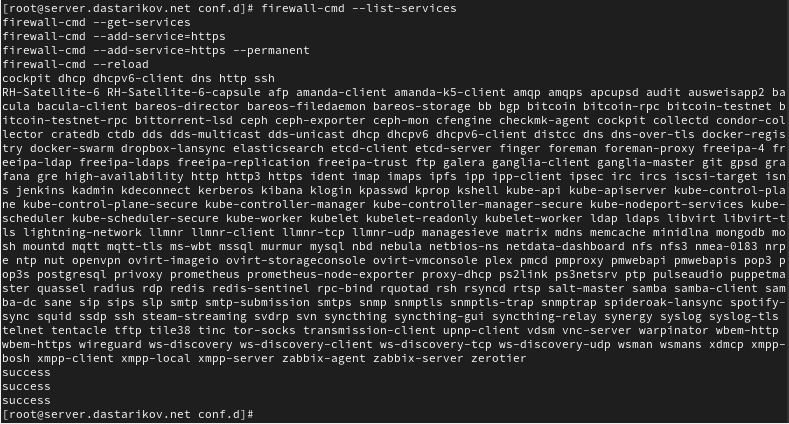
\includegraphics[width=\textwidth]{../images/image04.png}
    \captionof{figure}{Настройка межсетевого экрана.}
\end{frame}

\begin{frame}
\frametitle{Конфигурирование HTTP-сервера для работы через протокол HTTPS}
    \centering
    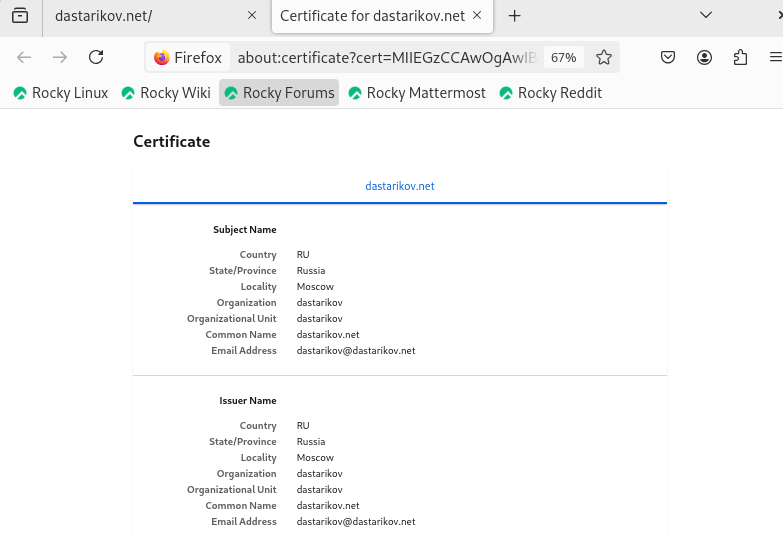
\includegraphics[width=\textwidth]{../images/image06.png}
    \captionof{figure}{Просмотр содержания созданного сертификата.}
\end{frame}


\begin{frame}
\frametitle{Конфигурирование HTTP-сервера для работы с PHP}
    \centering
    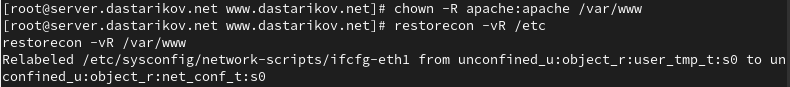
\includegraphics[width=\textwidth]{../images/image07.png}
    \captionof{figure}{Обновление контекста безопасности в SELinux.}
\end{frame}


\begin{frame}
\frametitle{Конфигурирование HTTP-сервера для работы с PHP}
    \centering
    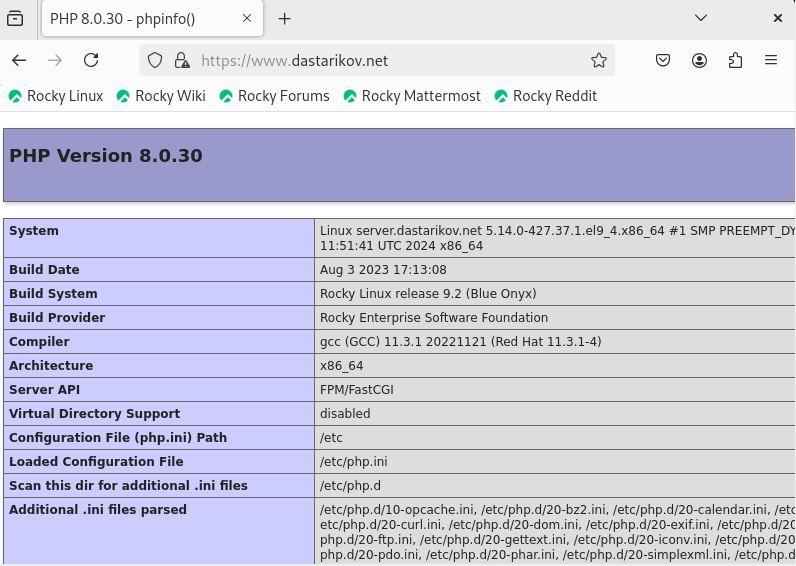
\includegraphics[width=\textwidth]{../images/image08.png}
    \captionof{figure}{Информация об оспользуемой на веб-сервере версии PHP.}
\end{frame}


\begin{frame}
\frametitle{Внесение изменений в настройки внутреннего окружения виртуальной машины}
    \centering
    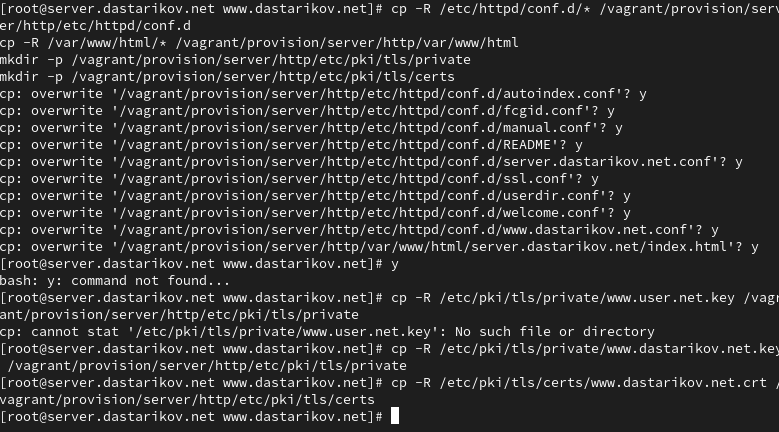
\includegraphics[width=\textwidth]{../images/image09.png}
    \captionof{figure}{Копирование конфигурационных файлов для настройки внутреннего окружения.}
\end{frame}

\begin{frame}[containsverbatim]
\frametitle{Внесение изменений в настройки внутреннего окружения виртуальной машины}
  \begin{minted}[fontsize=\small]{bash}
#!/bin/bash
echo "Provisioning script $0"
echo "Install needed packages"
dnf -y groupinstall "Basic Web Server"
dnf -y install php
echo "Copy configuration files"
cp -R /vagrant/provision/server/http/etc/httpd/* /etc/httpd
cp -R /vagrant/provision/server/http/var/www/* /var/www
chown -R apache:apache /var/www
restorecon -vR /etc
restorecon -vR /var/www
echo "Configure firewall"
firewall-cmd --add-service=http
firewall-cmd --add-service=http --permanent
firewall-cmd --add-service=https
firewall-cmd --add-service=https --permanent
echo "Start http service"
systemctl enable httpd
systemctl start httpd
  \end{minted}
\end{frame}



\begin{frame}
\frametitle{Выводы}
\begin{itemize}
    \item В результате выполнения лаборатрной работы приобрели практические навыки по расширенному конфигурированию HTTP-сервера Apache в части безопасности и возможности использования PHP.
\end{itemize}
\end{frame}
\end{document}
